\chapter{Description of Utilities in \numbers}
\label{c:numerics}

Each utility and the numerical algorithm used in the utility are
described in this chapter. Although most of the algorithms are
well-known and documented in several references, it is important to
understand the actual methods used in each of the utilities to avoid
misinterpretation of the output and to understand the limitations and
assumptions used to calculate the properties and values.

Another reason for describing the algorithms is that \numbers\ is
written as a basic shell program for reading \exo\ files.  If additional
utilities are developed for \numbers, it is likely that several of the
algorithms already implemented can be modified to perform the new
function.

This chapter is organized into several sections; each utility is
described in a separate section.  The descriptions include the function
of the utility and the algorithm used in the utility including its
assumptions and limitations.  The complete command syntax for each
utility is given in Section~\ref{sec:oper}; a summary of the command
syntax is given in Section~\ref{sec:opsum}.  Examples of the use of most
of the utilities are presented in Chapter~\ref{c:examples}.

\section{Mass Properties Utility}\label{sec:mass}

The mass properties utility calculates the volume, mass, mass moments of
inertia, and centroid location of the body.  These values are often
required in a finite element analysis to ensure that the finite element
idealization correctly approximates the actual body.  This utility also
lists the minimum, maximum, and average element volume for each material
block.  A summary of the equations used to calculate the mass properties
is given in this section.

The moments of inertia are originally calculated about the origin of the
coordinate system and then transferred to the centroid using the
parallel-axis theorem. The mass and the moments of inertia about the
origin of the coordinate system are given by the following integrals:
\begin{eqnarray}
 M      &=& \int_V \rho dV                         \label{V}\\
 I_x    &=& \int_V \rho\left(y^2 + z^2\right)\,dV \label{IX}\\
 I_y    &=& \int_V \rho\left(x^2 + z^2\right)\,dV \label{IY}\\
 I_z    &=& \int_V \rho\left(x^2 + y^2\right)\,dV \label{IZ}\\
 I_{xy} &=& \int_V \rho xy\,dV                    \label{IXY}\\
 I_{xz} &=& \int_V \rho xz\,dV                    \label{IXZ}\\
 I_{yz} &=& \int_V \rho yz\,dV                    \label{IYZ}
\end{eqnarray}

where $M$ is the mass, $\rho$ is the density, $I$ is the mass moment
of inertia, and the subscripts $x$, $y$, and $z$ denote the axes about
which the moment is measured.  The double subscripts indicate products
of inertia.  Note that the product of inertia with respect to any two
orthogonal axes is zero if either of the axes is an axis of symmetry.

\paragraph{Axisymmetric Two-dimensional Body:}
For an axisymmetric two-dimensional body, the integrals are written in
cylindrical coordinates using the radius $r$ and the angle $\theta$,
where $x = r\cos\theta$ and $z = r\sin\theta$.  The $y$-axis is assumed
to be the axis of revolution.  The infinitesimal volume $dV$ is equal to
$r\,dA\,d\theta$ where $dA$ is an infinitesimal area equal to $dr\,dy$.
Rewriting Equations \eref{V} through~\eref{IZ} in terms of
$r$ and $\theta$, and performing the theta integration from $-\pi$ to
$\pi$ gives:
\begin{eqnarray}
M   &=& 2\pi\rho\int_A r\,dA   \\
I_y &=& 2\pi\rho\int_A r^3\,dA   \\
I_x = I_z &=& 2\pi\rho\int_A r y^2\,dA + \pi\rho \int_A r^3\,dA\nonumber \\
    &=& 2\pi\rho\int_A r y^2\,dA + {I_y\over2}
\end{eqnarray}
The products of inertia $I_{xy}$, $I_{xz}$, and $I_{yz}$ are zero since
all three axes are symmetry axes.

\paragraph{Two-dimensional Planar Body:}
For a two-dimensional planar body, area moments of inertia are
calculated; the depth in the $z$-direction is ignored. The integrals
simplify as follows:
\begin{eqnarray}
 I_x    &=& \rho\int_A y^2\,dA                   \\
 I_y    &=& \rho\int_A x^2\,dA                   \\
 I_z    &=& \rho\int_A \left(x^2 + y^2\right)\,dA = I_x + I_y \\
 I_{xy} &=& \rho\int_A xy\,dA
\end{eqnarray}
The products of inertia $I_{xz}$ and $I_{yz}$ are both zero.

\paragraph*{Evaluation of Integrals:} The integrals are evaluated using
the isoparametric element formulation and Gaussian Quadrature. Details
of this process can be found in most books on finite element
methodology.  In \numbers, two options are available for integration of
the equations.  The two-dimensional equations can be integrated with
either 1- or 4-point quadrature, and the three-dimensional equations
with either 1- or 8-point quadrature.  The mass moments of inertia for
bodies with non-rectangular elements are calculated more accurately with
the higher-order integration; volumes and areas are integrated exactly
with either integration option.  The second-order quadrature rule is
also useful for calculating the section properties of a non-standard
shape.  For this purpose, the discretization of the body is only refined
enough to capture the essential details of the shape since a structural
analysis will not be performed.

\paragraph{Calculation of Centroid Location:} The location of the
centroid is calculated using the first mass moments about each of the
three coordinate axes.  The mass moments are summed in each of the three
coordinate directions over the range of the elements.  The centroid
location is then given by the quotient of the mass moment sums divided
by the total mass of the body.  For a two-dimensional axisymmetric body,
$x_c$ and $z_c$ (the $x$ and $z$ coordinates of the centroid) are zero;
for a two-dimensional planar body, $z_c$ is zero.

\section{Locate Utility}\label{sec:locate}

The locate utility outputs the numbers of all nodes or elements that are
within a specified distance from a user-defined point, line, or plane.
This information is often required for plotting results at a specified
location in the model, for example, the acceleration or velocity at the
centerline of a body during an impact analysis.  The equations used to
calculate the distances from a node or element centroid to the point,
line, or plane are defined in the following subsections.  All equations
are defined in terms of a three-dimensional body; for a two-dimensional
body the $z$ coordinates are deleted.

Note that the point location procedure is also a circle (2D) and sphere
(3D) location procedure and the line location procedure is also a
cylinder (3D) location procedure since the search interval distance from
the point and line can be specified.

In the location utility, the distance for an element is defined to be
the distance to the element geometric center. The location of the
element center is calculated by summing the four or eight nodal
coordinates in each coordinate direction and dividing by the number of
nodes.

\subsection{Point Location}\label{sec:plocate}
The point location utility outputs all nodes or elements that are a
specified distance from a user-specified point.  The distance $d_r$ from
the node or element to the point ($x_0$, $y_0$, $z_0$) is given by:
\begin{equation}
d_r = \sqrt{ (x_0-x_n)^2 + (y_0-y_n)^2 + (z_0-z_n)^2}
\end{equation}
where $x_n$, $y_n$, and $z_n$ are the coordinates of the node or
element.  The distance is calculated for each node or element and
compared to the user-specified distance and tolerance.  If the node or
element is within this range, its number and coordinates are output. The
angles $\theta$ and $\phi$ are also calculated.  The angle $\theta$ is
the angle between the $x$ axis and the projection of the line from the
point to the node onto the $x$--$z$ plane.  The angle $\phi$ is the
angle between the $y$ axis and the line from the point to the node.  In
two dimensions, $\theta$ is the angle between the line and the $x$ axis.
Figure~\ref{f:theta} illustrates the definitions of $\theta$ and $\phi$.

\begin{figure}
\centering
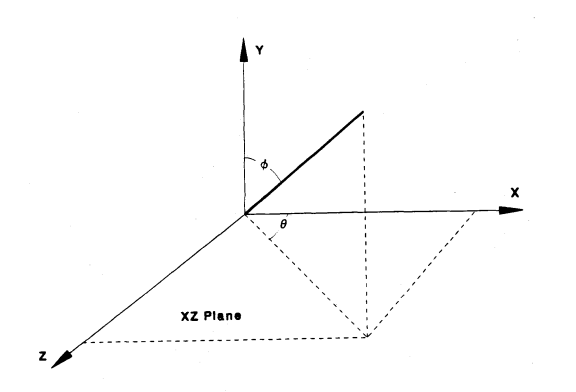
\includegraphics[scale=0.65]{figures/Angles.png}
\caption{Illustration of the Angles $\theta$ and $\phi$
for the Locate Point Utility}\label{f:theta}
\end{figure}

\subsection{Line Location}\label{sec:llocate}
The line location utility outputs all nodes or elements that are within
a specified distance from a user-specified line.  The distance is
measured normal to the line.   The parametric representation of the line
from $P_1$($x_1$, $y_1$, $z_1$) to $P_2$($x_2$, $y_2$, $z_2$) is $P(t) =
P_1 + (P_2 - P_1)t$.  The components of this line are:
\begin{equation}
\begin{array}{ccccc}
x &=& x_1 + (x_2 - x_1) t &=& x_1 + at   \\
y &=& y_1 + (y_2 - y_1) t &=& y_1 + bt   \\
z &=& z_1 + (z_2 - z_1) t &=& z_1 + ct   \\
\end{array}
\end{equation}
The minimum distance $d_t$ from the line to the point ($x_n$, $y_n$, $z_n$)
is
\begin{equation}
d_t^2 = (x_1+at-x_n)^2 +(y_1+bt-y_n)^2 +(z_1+ct-z_n)^2
\end{equation}
where the parameter $t$ is
\begin{equation}
t = -\frac{a(x_1-x_n) + b(y_1-y_n) +
c(z_1-z_n)}{a^2+b^2+c^2}\label{parametric}
\end{equation}

\subsection{Plane Location}\label{sec:slocate}
The plane location utility outputs all nodes or elements that are within
a specified distance from a user-specified plane.  The distance is
measured normal to the plane. A unique plane can be defined by a
specified point and a normal vector to the plane.  Given the point
($x_0$, $y_0$, $z_0$) and the unit vector $\vec{n} = a\vec{i} + b\vec{j} +
c\vec{k}$, the equation of the plane is:
\begin{eqnarray}
0 &=& ax + by + cz + d      \label{plane} \\
d &=& -( ax_0 + by_0 + cz_0 )
\end{eqnarray}
The normal distance $d_n$ from the plane to a node or
element center is:
\begin{equation}
d_n = \frac{\left| a x_n + b y_n + c z_n - d\right|}%
                                    {\sqrt{a^2 + b^2 + c^2}}
\end{equation}
where the subscript $n$ refers to the coordinates of the node or
element.  The normal distance is calculated for each node or element and
compared to the user-specified distance and tolerance.  If the node or
element is within this range, its number, coordinates, normal distance,
and radial distance are output.  The radial distance is the same
distance calculated in the point location utility.

\subsection{Sort Algorithm}

Although sort is not a location option, it is used in the location
utility to order the output.  \numbers\ uses the {\em heapsort} routine
which has been recommended in Reference~\cite{Press:nr} as a good
routine for a variety of sorting applications.  It is an ``in-place''
sort requiring no auxiliary storage.  It is an $N\log_2N$ process, not
only on average, but also for worst-case order of input data.  A FORTRAN
listing of the sort subroutine is given in Appendix~\ref{a:sort}.  One
disadvantage of the sort routine is that it is not ``stable.''  This
means that sorting the data a second time on a different field will
destroy the order of the first sort.  A method for sorting on two or
more fields simultaneously is being investigated and will be implemented
in a later version of \numbers.

\subsection{Sort Fields}\label{sortfields}

The output from the location utility can be sorted on any of the
calculated quantities or ``fields.''  The table below lists the fields
that are defined for each of the location options; these are defined
following the table.

\begingroup\small
\tabcolsep=3pt
\begin{center}
%\begin{tabular}{|>{\sf}l|c|  *{8}{>{\sf}l}|  }\hline
\begin{tabular}{|l|c|  *{8}{l}|  }\hline
\rm Option  &2D/3D &\multicolumn{8}{|c|}{\rm Valid \param{sort\_fields}}\\
\hline\hline
POINT  & 2D &  X  &  Y  &     &   & DISTANCE &            & THETA &     \\
POINT  & 3D &  X  &  Y  &  Z  &   & DISTANCE &            & THETA & PHI \\
LINE   & 2D &  X  &  Y  &     & T & DISTANCE & PARAMETRIC &       &     \\
LINE   & 3D &  X  &  Y  &  Z  & T & DISTANCE & PARAMETRIC &       &     \\
PLANE  & 3D &  X  &  Y  &  Z  &   & DISTANCE &            & RADIUS&     \\
\hline
\end{tabular}
\end{center}
\endgroup

\def\descriptionlabel #1{\sf #1:\hfil}
\begin{description}
\item[X, Y, {\rm or} Z] The \cmd{x}, \cmd{y}, or \cmd{z} coordinate
of the located node or element center.
\item[T] The parametric distance from the initial point of the line to
the located node or element center as defined in
Equation~\eref{parametric}.  The initial point of the line is located at
\cmd{T} = 0; the final point is located at \cmd{T} = 1.
\item[PARAMETRIC] The same quantity as \cmd{T}.
\item[DISTANCE] The distance from the node or element center to the
location point, line, or plane.  See the respective sections above for
the definition of distance for each of the location options.
\item[RADIUS] The shortest distance from the plane definition point (see
Section~\ref{sec:slocate}) to the located node or element center.
\item[THETA] For three-dimensional bodies, \cmd{THETA} is the angle
between the $x$ axis and the projection of the line from the point to
the node or element center onto the $x$--$z$ plane (see
Section~\ref{sec:plocate}).  For two-dimensional bodies, \cmd{theta} is
the angle between the line from the point to the node or element center
and the $x$ axis.
\item[PHI] The angle between the $y$ axis and the line from the point to
the located node or element center.
\end{description}

\section{Cavity Volume Utility}\label{sec:cavity}
The cavity volume utility calculates the volume and change in volume of
a cavity or hole in a body.  The boundary of the cavity is defined by
side set flags in the \exo\ file.  Two separate calculations are
involved in this utility; the first is the calculation of the
cavity volume, and the second is the calculation of the change in
volume.

The cavity volume is calculated by forming triangles (2D) or
pentahedrons (3D) for each segment of the cavity boundary.  The apex of
the triangles or pentahedrons are at a user-specified point. The bases
of the triangles or pentahedrons are the segments of the cavity boundary
side set.  The segments are element faces; in two-dimensions, the faces
are lines; in three-dimensions, the faces are four-node quadrilaterals.
The faces are assumed to be planar.  The volume of each triangle or
pentahedron is calculated and the sum of the volumes is, for certain
geometries, the volume of the cavity.

Figure~\ref{cvol2d} is an example of this process for a two-dimensional
cavity with three boundary segments: 1--2, 2--3, and 3--4.
\begin{figure}
\centering
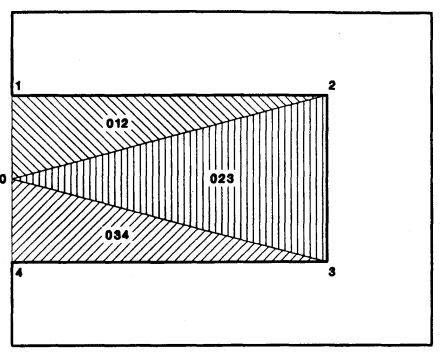
\includegraphics[scale=0.75]{figures/Cavity.png}
\caption{Illustration of Cavity Volume Determination for
a Two-Dimensional Cavity}\label{cvol2d}
\end{figure}
The area is calculated by summing the areas of the three triangles
{\sf012}, {\sf023}, and {\sf034}, where the three numbers refer to the
points defining the triangle and point {\sf0} is the apex or center
point. A similar process is used for three-dimensional cavities except
that pentahedral volumes are calculated instead of triangular areas. The
volume $V$ of a pentahedron with the apex at the point $(x_c,y_c,z_c)$
and the base formed by a boundary segment is~\cite{flanagan}:
\begin{eqnarray}
V = &\frac{1}{12}&\{
 ((2y_c - y_3) z_{42} + y_2 (z_{c3} + z_{c4}) - y_4 (z_{c3} + z_{c2})) x_1 \nonumber \\
&+& \phantom{\{}((y_4 - 2y_c) z_{31} + y_3 (z_{c4} + z_{c1}) - y_1 (z_{c4} + z_{c3})) x_2 \nonumber \\
&+& \phantom{\{}((y_1 - 2y_c) z_{42} + y_4 (z_{c1} + z_{c2}) - y_2 (z_{c4} + z_{c1})) x_3 \nonumber \\
&+& \phantom{\{}((2y_c - y_2) z_{31} + y_1 (z_{c2} + z_{c3}) - y_3 (z_{c2} + z_{c1})) x_4 \nonumber \\
&+& \phantom{\{}(y_{24}   z_{31} + y_{31} z_{42})  2  x_c\}
\end{eqnarray}
where the numerical subscript refers to the sequence of the node of the
boundary segment, the $c$ subscript refers to the center location, and
the double subscript $z_{ij}$ is defined as $z_i-z_j$.

The planar area $V_P$ of a triangle with the apex at the point
$(x_c,y_c)$ and the base formed by a boundary segment is:
\begin{equation}
V_P = \sfrac{1}{2}[(y_1-y_c) (x_2-x_c) - (y_2-y_c) (x_1-x_c)]
\end{equation}
where the subscript refers to the first and second node of the boundary
segment, and $y_c$ is the approximate vertical geometric center of the
cavity. It is calculated by summing the $y$ coordinates and dividing by
the total number of nodes on the boundary.

If the body is axisymmetric, the volume $V_A$ is calculated as:
\begin{eqnarray}
x_c &=& \sfrac{1}{3}(x_1 + x_2) \nonumber \\
V_A &=& 2\pi x_c V_P
\end{eqnarray}
where $V_P$ is the area calculated for the plane strain cavity.

The above method correctly calculates the volume of cavities defined by
a closed boundary.  However, many cavities are bounded on one or more
sides by symmetry planes which are not included in the cavity boundary
definition.  In two dimensions, the correct volume will be calculated if
the triangle apex is on the axis of symmetry.  In three dimensions, the
correct volume will be calculated if the apex of the pentahedron is on
the symmetry plane, or if it is on the intersection of two or more
symmetry planes.  If the apex point is not specified  by the user, it is
set to the point $(0,0,0)$ for three-dimensional bodies, and the point
$(0,y_c)$ for two-dimensional bodies, where $y_c$ is the approximate
vertical geometric center of the cavity.

\paragraph*{Cavity Volume Change:}
The change in cavity volume is calculated by calculating the volume of
the hexahedron formed by the original element face and the displaced
element face.  This is repeated for each element face on the cavity
boundary and the total volume change is the sum of the element face
volume changes.  Note that this calculation is correct for all cavities
even if they are bounded by symmetry planes.

For a three-dimensional cavity, the volume change $\Delta V$ for each
element on the cavity boundary is given by the following sequence of
calculations~\cite{PRONTO3D}.
\begin{equation}
\Delta V = \sfrac{1}{12}\sum_{i=1}^8 x_i B_i
\end{equation}
where $x_i$ for $i\le 4$ is the $x$ coordinate of a node on the element
face and $x_i$ for $5 \le i\le 8$ is the displaced coordinate of node
$i-4$.  The $B_i$ values are given by:
\begin{eqnarray*}
B_{1} &=&   y_2 (z_{63}-z_{45}) + y_3 z_{24} + y_4 (z_{38}-z_{52})
          + y_5 (z_{86}-z_{24}) + y_6 z_{52} + y_8 z_{45} \\
B_{2} &=&   y_3 (z_{74}-z_{16}) + y_4 z_{31} + y_1 (z_{45}-z_{63})
          + y_6 (z_{57}-z_{31}) + y_7 z_{63} + y_5 z_{16} \\
B_{3} &=&   y_4 (z_{81}-z_{27}) + y_1 z_{42} + y_2 (z_{16}-z_{74})
          + y_7 (z_{68}-z_{42}) + y_8 z_{74} + y_6 z_{27} \\
B_{4} &=&   y_1 (z_{52}-z_{38}) + y_2 z_{13} + y_3 (z_{27}-z_{81})
          + y_8 (z_{75}-z_{13}) + y_5 z_{81} + y_7 z_{38} \\
B_{5} &=&   y_8 (z_{47}-z_{61}) + y_7 z_{86} + y_6 (z_{72}-z_{18})
          + y_1 (z_{24}-z_{86}) + y_4 z_{18} + y_2 z_{61} \\
B_{6} &=&   y_5 (z_{18}-z_{72}) + y_8 z_{57} + y_7 (z_{83}-z_{25})
          + y_2 (z_{31}-z_{57}) + y_1 z_{25} + y_3 z_{72} \\
B_{7} &=&   y_6 (z_{25}-z_{83}) + y_5 z_{68} + y_8 (z_{54}-z_{36})
          + y_3 (z_{42}-z_{68}) + y_2 z_{36} + y_4 z_{83} \\
B_{8} &=&   y_7 (z_{36}-z_{54}) + y_6 z_{75} + y_5 (z_{61}-z_{47})
          + y_4 (z_{13}-z_{75}) + y_3 z_{47} + y_1 z_{54}
\end{eqnarray*}
where $y_i$ and $z_i$ are defined in the same way as $x_i$, and $z_{ij}$
is equal to $z_i - z_j$.

For a two-dimensional, planar cavity, the volume change $\Delta V_P$ for
each element on the cavity boundary is equal to
\begin{equation}
\Delta V_P = \sfrac{1}{2}\left[x_{12} (\Delta y_2 + \Delta y_1) -
           y_{12} (\Delta x_2 + \Delta x_1) +
           \Delta x_1 \Delta y_2 -
           \Delta x_2 \Delta y_1\right]
\end{equation}
where $x$ and $y$ are the original coordinates of the face nodes and
$\Delta x$ and $\Delta y$ are the $x$ and $y$ displacements of the
nodes.

For an axisymmetric cavity, the volume change $\Delta V_A$ for each
element on the cavity boundary is equal to
\begin{equation}
\Delta V_A = 2\pi x_c \Delta V_P
\end{equation}
where $x_c$ is the $x$ coordinate of the geometric center which is equal
to
\begin{equation}
x_c = \frac{(\Delta x_2 + \Delta x_1)}{4} +
      \frac{(x_2 + x_1)}{2}
\end{equation}

\section{Overlap Utility}\label{sec:overlap}

The overlap utility is intended to assist the analyst in the generation
of a mesh with valid contact surfaces.  One of the most difficult tasks
in generating a valid contact surface occurs when the contact surface is
curved with different discretizations on the two surfaces.  In this
case, a small gap must be inserted between the surfaces to prevent
penetration. Figure~\ref{f:overlap} illustrates the problem that can
occur if the gap is not large enough or nonexistent. Note that the nodes
on the more refined side of the contact surface penetrate the elements
on the other side of the surface.  This is a somewhat contrived example
to illustrate the problem; in actual finite element meshes it is very
difficult to notice the overlap unless the mesh is examined element by
element. However, if an analysis is run with overlapping contact
surfaces, the problem manifests itself in a sudden increase in kinetic
energy or by excessive deformations and velocities in the overlapped
portion of the mesh since the code will separate the contact surface in
one timestep.  Currently, the utility only checks for penetration of the
master surface by the slave surface; however, other checks for valid
contact surfaces, such as continuity or other requirements imposed by
analysis codes, can be added if there is a need.

\begin{figure}
\centering
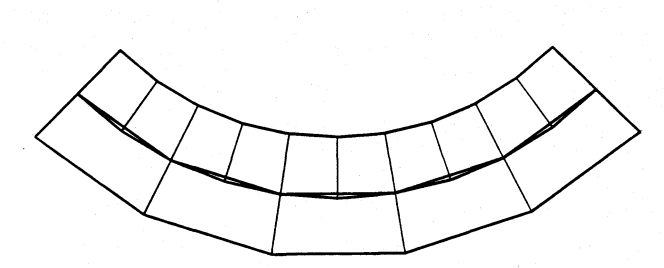
\includegraphics[scale=0.5]{figures/Overlap.png}
\caption{Illustration of Contact Surface Overlap due to
Discretization Mismatch on Curved Contact Surfaces}
\label{f:overlap}
\end{figure}

Many times, the most efficient method to determine whether the contact
surfaces overlap is to run the analysis for a very short period of time,
and then examine the results to see if the kinetic energy has increased
suddenly, or if the mesh has been ``blown'' apart where the analysis
code detects an overlapping contact surface and separates it in one
timestep---both symptoms indicate that a slideline overlap exists in the
original mesh.

The overlap utility was written to provide an efficient means of
determining whether an overlap exists prior to running an analysis. The
algorithm is logically broken into three separate steps. In the first
step, a ``bounding box'' is defined for each element on the master
surface.  The bounding box contains the coordinate ranges in each of the
coordinate directions.   Secondly, for each element on the master
surface, each node on the slave surface is tested to determine if it is
within the bounding box.  This test is a simple comparison of the slave
node coordinates with the coordinates of the bounding box.  Finally, if
a node is within an element's bounding box, the more computationally
expensive calculation of determining whether the node penetrates the
element is performed.  To determine if the node penetrates the element,
four triangles (two-dimensional body) or six pentahedrons
(three-dimensional body) are formed with the slave node as the apex and
each element face as the base.  The volume of each triangle or
pentahedron is calculated; if all of the volumes are positive, the node
is inside the element; if a volume is equal to zero, the node is on
the face. If the node is inside the element, its node number and the
number and connectivity of the penetrated element are output.  At the
end of the calculation, the total number of nodes penetrating the
surface and the number of nodes on the surface are output.

The volume $V_P^i$ of the three-dimensional pentahedron formed by
slave node $s$ and the element face $i$ is equal
to~\cite{flanagan}:
\begin{eqnarray}
12V_P^i &=& \phantom{{}+{}}x_A[(2y_S - y_C)  z_{DB} + y_B  (z_{SC} + z_{SD}) -
     y_D  (z_{SC} + z_{SB})] \nonumber \\
&\ &  {}  + x_B[(y_D - 2y_S)  z_{CA} + y_C  (z_{SD} + z_{SA})-
     y_A  (z_{SD} + z_{SC})] \nonumber \\
&\ &  {}  + x_C[(y_A - 2y_S)  z_{DB} + y_D  (z_{SA} + z_{SB})-
     y_B  (z_{SD} + z_{SA})] \nonumber \\
&\ &  {}  + x_D[(2y_S - y_B)  z_{CA} + y_A  (z_{SB} + z_{SC})-
     y_C (z_{SB} + z_{SA})] \nonumber \\
&\ &  {}  + 2x_S[y_{BD} z_{CA} + y_{CA} z_{DB} ]
\end{eqnarray}
where the subscript $S$ refers to the slave node, and the subscripts
$A$, $B$, $C$, and $D$ refer to the nodes on an element face (assumed to
be planar) as given in Table~\ref{t:nodes}.

\begin{table}
\parbox[t]{3.0in}{
\begin{center}
\begin{tabular}{l|cccccc}
\multicolumn{7}{c}{Hexahedron} \\
\multicolumn{7}{c}{\ } \\
  & \multicolumn{6}{c}{Face} \\
  & 1 & 2 & 3 & 4 & 5 & 6 \\ \hline
A & 1 & 6 & 6 & 5 & 4 & 1 \\
B & 2 & 7 & 5 & 1 & 3 & 5 \\
C & 3 & 3 & 8 & 4 & 7 & 6 \\
D & 4 & 2 & 7 & 8 & 8 & 2 \\
\end{tabular}
\end{center}}\hfil
\parbox[t]{3.0in}{
\begin{center}
\begin{tabular}{l|cccc}
\multicolumn{5}{c}{Quadrilateral} \\
\multicolumn{5}{c}{\ } \\
  & \multicolumn{4}{c}{Face} \\
  & 1 & 2 & 3 & 4 \\ \hline
A & 1 & 2 & 3 & 4 \\
B & 2 & 3 & 4 & 1 \\
\end{tabular}
\end{center}}
\caption{Numbering of Face Nodes on an Eight-Node Hexahedral Element and
a Four-Node Quadrilateral Element}\label{t:nodes}
\end{table}

The volume $V_T^i$ of the two-dimensional triangle formed by the
slave node $s$ and the element face $i$ is equal to:
\begin{equation}
2V_T^i = x_A (y_B - y_S) + x_B (y_S - y_A) + x_S (y_A - y_B)
\end{equation}
where the subscript $S$ refers to the slave node, and the subscripts
$A$ and $B$ refer to the nodes on an element face as given in
Table~\ref{t:nodes}.

\section{Time Step Estimation Utility}\label{sec:timestep}

Explicit integration is used in most large-deformation, nonlinear,
transient dynamics finite element codes, for example
\code{PRONTO}~\cite{PRONTO2D,PRONTO3D}. This utility provides an
estimate of the time step size which will be used in the explicit
integration in these codes.

The stable time step $\Delta t$ for the central difference operator
commonly used in transient dynamic analysis codes is given
by~\cite{Cook}
\begin{equation}
\Delta t \leq {2\over \omega_{\max}} \left(\sqrt{1+\epsilon^2} -
\epsilon\right)
\end{equation}
where $\omega_{\max}$ is the maximum frequency of the mesh, and
$\epsilon$ is the fraction of critical damping in the highest element
mode.  In a explicit integration finite element code, the linear bulk
viscosity term is an estimate of $\epsilon$~\cite{PRONTO2D}. The default
value of $\epsilon$ is 0.06 which is the default value of the linear
bulk viscosity used in \code{PRONTO2D} and \code{PRONTO3D}.

Flanagan and Belytschko~\cite{flanagan} have derived simple
formulas for bounding the maximum eigenvalues for the uniform strain
eight-node hexahedron and four-node quadrilateral which can be used to
provide conservative estimates of the maximum frequency.  The maximum
frequency estimate for a rectangular quadrilateral element is
\begin{equation}
\hat\omega_{\max}^2 = {4(\lambda + 2\mu)\over\rho}\left({1\over s_1^2} +
   {1\over s_2^2}\right)
\end{equation}
where $s_1$ and $s_2$ are the lengths of the sides of the rectangle,
$\lambda$ and $\mu$ are Lame's constants, $\rho$ is the density, and
$\hat\omega_{\max}$ is the predicted value for the maximum frequency.
Similarly, for a rectangular parallelepiped hexahedron,
\begin{equation}
\hat\omega_{\max}^2 = {4(\lambda + 2\mu)\over\rho}\left({1\over s_1^2} +
   {1\over s_2^2}+{1\over s_3^2}\right)
\end{equation}

Substituting the maximum frequency equation into the stable time step
equation gives the following estimate for the stable time step size:
\begin{equation}
\Delta\hat t\le \sqrt{\frac{\rho}{\lambda+2\mu}}
      \left(\sum_{i=1}^{n_D}\frac{1}{s_i^2}\right)^{-1/2}
      \left(\sqrt{1+\epsilon^2} - \epsilon\right)
\end{equation}
where $\Delta\hat t$ is the estimate of the stable time step, and $n_D$
is the number of dimensions.  The first quantity on the right-hand side
of the inequality is the inverse of the dilatational wave speed which is
input by the user.  The second quantity is calculated by \numbers\ with
the assumption that the element is rectangular.

The output from this utility includes the calculated time step, the
element with the minimum time step, and the number of time steps per
millisecond of analysis time for each element block.

The number of time steps per millisecond can be used to estimate the
computer time required to perform an analysis.  Most explicit transient
dynamics codes output the average CPU time required to perform the
calculations for one element for one time step. Although this quantity
varies for different constitutive models and the number of contact
surfaces (slidelines), the average value is usually relatively constant
and well known.  The CPU time per millisecond of analysis time can be
estimated using the formula
\begin{equation}
{CPU\over ms} = \left(10^{-3}\over \Delta\hat t\right)
                ({\sf Speed})({\sf NUMEL})
\end{equation}
where {\sf NUMEL} is the number of elements, {\sf Speed} is the CPU time
per element per timestep, and $(10^{-3}/\Delta\hat t)$ is the number of
time steps per millisecond.

\section{Gap Utility}\label{sec:gap}

The gap utility is used to determine the distance between nodes on two
surfaces.  One surface is called the ``master'' surface and the other
surface is the ``slave'' surface.  For each node on the master surface,
a normal vector is calculated as shown below.  A matching process is
then performed to determine the ``closest'' slave node to each master
node, where closeness can be defined either as closest to the master
node normal vector, or closest in absolute distance.  Figure~\ref{f:gap}
illustrates the two closeness measures.  In this figure, Node~$M$ is the
master node and nodes $S_1$ and~$S_2$ are two slave nodes.  If the
absolute distance is used, node~$S_1$ will be the matching node; if the
distance to the normal vector is used, node~$S_2$ will be the matching
node.

\begin{figure}
\centering
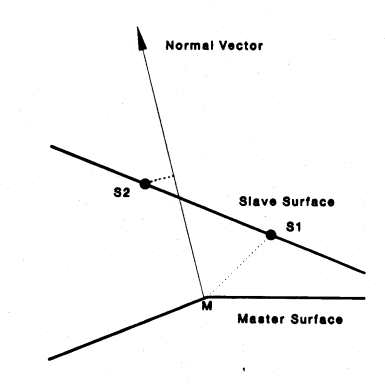
\includegraphics[scale=0.65]{figures/Gap.png}
\caption{Illustration of Closeness Measures Used in the Gap Utility}
\label{f:gap}
\end{figure}

After all of the nodes on the master surface have been matched to a node
on the slave surface, the normal and tangential distances, measured in
the coordinate frame of the normal vector, are determined for the
undeformed geometry and for each of the selected timesteps in the
database.  This utility is normally used to calculate the change in
distance between two surfaces, for example, the closure of a drift in a
geomechanics problem or the slip (tangential movement) along a contact
surface.

The normal for a node is defined to be the average normal of the element
faces for all elements connected to the node.  For a three-dimensional
body, a technique developed by Newell~\cite{Rogers:pefcg} gives the
exact normal for planar faces and a ``best'' approximation for almost
planar faces. The coefficients $a$, $b$, and $c$ of the normal vector
for an element face $\vec{n} = a\vec{i} + b\vec{j} + c\vec{k}$ are given by:
\begin{eqnarray}
a &=& \sum_{i=1}^n (y_i - y_j)(z_i + z_j) \nonumber\\
b &=& \sum_{i=1}^n (z_i - z_j)(x_i + x_j) \label{3dnorm}\\
c &=& \sum_{i=1}^n (x_i - x_j)(y_i + y_j) \nonumber
\end{eqnarray}
where $n$ is the number of nodes per face, and $j = 1$ if $i=n$, or
$j=i+1$ if $i\ne n$.  The vector is then normalized and added to the
direction cosine matrix for each node on the face.  After all of the
element normals have been computed and added to the direction cosine
matrix, the average direction cosine unit vector for each node is
determined by normalizing each entry in the direction cosine matrix.

The procedure is similar for a two-dimensional body, except that the
normal vector for an element face $\vec{n} = a\vec{i} + b\vec{j}$ is given by:
\begin{eqnarray}
      r &=& \sqrt{(x_i - x_j)^2 + (y_i - y_j)^2} \nonumber \\
      a &=& (x_i - x_j) / r                      \label{2dnorm}\\
      b &=& (y_i - y_j) / r                      \nonumber
\end{eqnarray}
where $x_i$ and $x_j$ are the $x$ coordinates of the two face nodes, and
$y_i$ and $y_j$ are the $y$ coordinates of the two face nodes.

After the average nodal normals have been calculated, the node matching
process is performed.  For each node on the master surface, the {\em
closest} node on the slave surface is determined.  There are two
criteria for determining closeness: radial distance and tangential
distance.  The radial distance $d_r$ between two nodes is simply
\begin{equation}
d_r = \sqrt{(x_s - x_m)^2 + (y_s - y_m)^2 + (z_s - z_m)^2}\label{distr}
\end{equation}
where $x$, $y$, and $z$ are the nodal coordinates and the subscripts $m$
and $s$ refer to the master and slave nodes, respectively.

The tangential distance is the distance from the master node's normal
vector to the slave node.  The distance is given by~\cite{Rogers:pefcg}:
\begin{eqnarray}
d_t &=& \sqrt{d_r^2 - d_n^2}\label{distt}  \\
d_n &=& -\left(a(x_m - x_s) + b(y_m - y_s)+c(z_m-z_s)\right)\label{distn}
\end{eqnarray}
where $d_r$ is the radial distance given in Equation~\eref{distr}, $d_n$
is the distance to the slave node measured in the direction of the
normal vector, and $a$, $b$, and $c$ are the components of the unit
normal vector determined in Equations \eref{3dnorm} or~\eref{2dnorm}.

\section{Limits Utility}

The limits utility provides the basic function of determining the
minimum, maximum, and range of the coordinates for each of the material
blocks.  No special algorithms are used in this utility and there are no
inherent limitations or assumptions in its implementation. The utility
simply examines the coordinates of each element in each element block
and saves the minimum and maximum values.  After all of the elements
have been processed, the minimum and maximum values are subtracted to
determine the coordinate range of the data.
